\section{VC Dimensions}
\label{sec:vc-dimension}
\begin{enumerate}
\item ~[10 points] Suppose you have a finite hypothesis space
  $\mathcal{C}$. Show that its VC dimension at most
  $\log_2|\mathcal{C}|$ (Hint: You also prove this by contradiction.)

The growth function $m_\mathcal{C}(N)$ for a hypothesis class $\mathcal{C}$ is defined as the maximum number of dichotomies than can be generated by $\mathcal{C}$ on any $N$ points. 

The VC dimension of $\mathcal{C}$,$d_{VC}(\mathcal{C})$, is the largest $N$ for which $m_\mathcal{C}(N)=2^N$. In other words, $d_{VC}(\mathcal{C})$ is the largest $N$ that can be split into all possible dichotomies by the hypothesis class $\mathcal{C}$.

Each hypothesis in the hypothesis class $\mathcal{C}$ can at the maximum generate a distinct dichotomy. That means, there could be a maximum of $\left | \mathcal{C} \right| $ dichotomies that can be generated by the hypothesis class $\mathcal{C}$.

This means that $d_{VC}(\mathcal{C})$ is the largest $N$ such that 

\begin{equation*}
\begin{aligned}
m_\mathcal{C}(N)=2^N &= \left | \mathcal{C} \right| \\
N \log_2 2 &= \log_2 \left | \mathcal{C} \right| \\
N &= \log_2|\mathcal{C}|
\end{aligned}
\end{equation*}

This means that the VC dimension at most $\log_2|\mathcal{C}|$

\item ~[10 points] Given some finite domain set, $\mathcal{X}$, and a
  number $k \leq |\mathcal{X}|$, figure out the VC-dimension of each
  of the following classes and prove your claims:

  \begin{enumerate}
  \item
    $\mathcal{H}_{=k}^{\mathcal{X}} = \{h \in \{0,1\}^\mathcal{X} :
    |{x : h(x) = 1} | = k \}$. That is , the set of all functions that
    assign the value 1 to exactly $k$ elements of $\mathcal{X}$.

  \item $\mathcal{H}_{\leq k}^{\mathcal{X}} = \{h \in
    \{0,1\}^\mathcal{X} : |{x : h(x) = 1} | \leq k \quad or \quad |{x
      : h(x) = 0} | \leq k\}$. That is , the set of all functions that
    assign the value 1 or 0 to at most $k$ elements of $\mathcal{X}$.

  \end{enumerate}

\item ~[10 points] Suppose we have an instance space consisting of
  real numbers and a hypothesis space $\mathcal{H}$ consisting of {\em
    two} disjoint intervals, defined by $[a, b]$ and $[c, d]$. That
  is, a point $x \in \Re$ is labeled as positive if, and only if,
  either $a \leq x \leq b$ or $c \leq x \leq d$. Determine the VC
  dimension of $\mathcal{H}$?


\item ~[15 points] We have a learning problem where each example is a
  point in $\Re^2$. The concept class $H$ is defined as follows: A
  function $h \in H$ is specified by two parameters $a$ and $b$. An
  example ${\bf x} = \{x_1, x_2\}$ in $\Re^2$ is labeled as $+$ if and
  only if $x_1 + x_2 \geq a$ and $x_1 - x_2 \leq b$ and is labeled $-$
  otherwise.

  For example, if we set $a = 0, b = 0$, the grey region in figure
  \ref{f1} is the region of ${\bf x} = \{x_1, x_2\}$ that has label
  $+1$.

  \begin{figure}[h!]
    \centering
    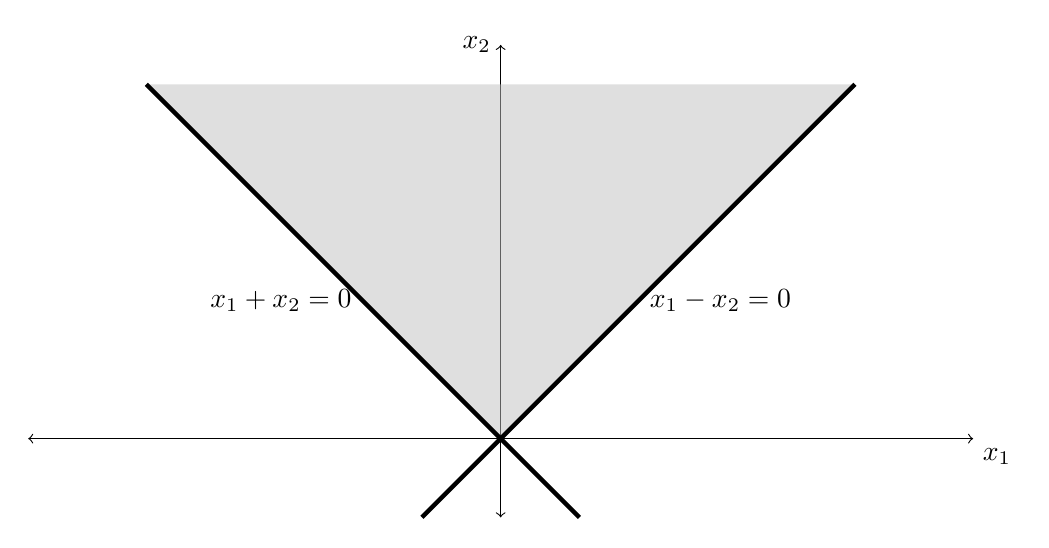
\begin{tikzpicture}[domain=0:2]
      \draw[<->] (-6,0) -- (6,0) node[below right] {$x_1$};
      \draw[<->] (0,-1) -- (0,5) node[left] {$x_2$};
      \fill[gray!50,opacity=0.5] (0,0) -- (4.5,4.5) -- (-4.5,4.5) -- (0,0);
      \draw [ultra thick] (4.5,4.5) -- node [midway,right] {$x_1 -x_2 = 0$} (-1,-1);
      \draw [ultra thick] (-4.5,4.5) --  node [midway,left] {$x_1 + x_2 = 0$}(1,-1);
    \end{tikzpicture}
    \caption{An example with $a = 0, b = 0$. All points in the gray region
      (extending infinitely) shows the region that will be labeled as
      positive.} \label{f1}
  \end{figure}



  What is the VC dimension of this class?


\item ~[{\bf For 6350 Students,} 15 points] Let two hypothesis classes
  $H_1$ and $H_2$ satisfy $H_1 \subseteq H_2$. Prove: $VC(H_1) \leq
  VC(H_2)$.

\end{enumerate}
%%% Local Variables:
%%% mode: latex
%%% TeX-master: "hw"
%%% End:
